% \pagebreak[4]
% \hspace*{1cm}
% \pagebreak[4]
% \hspace*{1cm}
% \pagebreak[4]

% --- here we need to update:
% 1. references [done][need to double check]
% 2. formulas [done][need to double check]
% 3. figures [done][checked, but keep paying attention to the size]
% 4. figure captions [done][need to double check this]
% 5. figure references [done][need to double check]

\chapter{Cortical Organization of Binocular Disparity in Human Visual Area V3A}
\ifpdf
    \graphicspath{{chapter4/chapter4-figs/PNG/}{chapter4/chapter4-figs/PDF/}{chapter4/chapter4-figs/}}
\else
    \graphicspath{{chapter4/chapter4-figs/EPS/}{chapter4/chapter4-figs/}}
\fi

\renewcommand{\runningTitle}{Cortical organization for binocular disparity}
\markboth{\MakeUppercase{\thechapter. \runningTitle }}{\thechapter. \runningTitle}

This chapter reproduces the work associated with the following published manuscript: 

Goncalves NG \textit{et al.}. 7 Tesla fMRI Reveals Systematic Functional Organization for Binocular Disparity in Dorsal Visual Cortex. \textit{Journal of Neuroscience}, 35(7), 3056--3072. 2015.

The content of the present chapter mirrors the content of the publication above. However, the citation style and references to figures and equations have been adjusted such that they are consistent with the fellow chapters of the thesis.

This project stemmed out of a collaboration with several other researchers, namely Dr. Hiroshi Ban, Dr. Rosa Sanchez-Panchuelo, Dr. Susan T. Francis, Dr. Denis Schl\"{u}ppeck and Dr. Andrew E. Welchman . Dr Sanchez-Panchuelo, Dr. Francis and Dr. Schl\"{u}ppeck designed and assisted with magnetic resonance imaging data collection at the University of Nottingham. Dr. Ban implemented visual stimulation protocols for pilot experiments and contributed to the analysis of pilot data. All the authors contributed to the experimental design of the study and to manuscript writing. 

All the visual stimulation procedures and magnetic resonance imaging data analyses reported below were performed by me, under supervision of the remaining authors.


\section{Introduction}

Understanding cortical organization at the mesoscopic scale is an important step in characterizing local neural circuits. The hypercolumn concept \cite{Hubel:1974sv} has been extremely influential in modeling cortical functional architecture \cite{Tso:2009tg}, and provides a framework to test the neural machinery that facilitates sensory processing. However, despite good knowledge from animal models, comparatively little is known about the local architecture of human cortex. 

Here I investigate the brain organization that may underlie our ability to make precise depth judgments based on binocular disparities. Extracting depth from disparity is a demanding, yet routine, neural computation, making it plausible that it is supported by systematically organized cortical structures. In particular, I question if --- and where --- responses of neural populations in close proximity share similar characteristics. Such spatial organization is often interpreted as an index for cortical specialization \cite{DeAngelis:1999fk, Chen:2008vn}.

Evidence from neurophysiology suggests that areas in extrastriate cortex exhibit some form of cortical organization. Most notably, DeAngelis and Newsome performed tangential electrode penetrations and discovered a gradual shift in binocular disparity preference with the extent of the penetration \cite{DeAngelis:1999fk}. Effectively, this suggests that nearby neurons in MT respond to binocular disparity in a similar fashion, and that those response properties vary smoothly along the cortex. However, when electrode penetrations were performed perpendicular to the cortex (i.e. along the cortical column), DeAngelis and Newsome observed little variation in disparity selectivity, demonstrating the existence of cortical columns for binocular disparity. Further recordings from cat and macaque cortex also support this idea: i.e., electrophysiology and optical imaging showed that disparity populations are structured in V2 \cite{Hubel:1987ly,Roe:1995ys,Tso:2001zr,Chen:2008vn,Kara:2009fk}, V3/V3A \cite{Adams:2001wt,Anzai:2011gb,Yeagle_Lafer-Sousa_Conway_2013}. By contrast, area V1 is reported to show, at best, weak clustering \cite{LeVay:1988ve,Prince:2002cr}.

Tests of disparity processing in the primate brain point to strong and informative fMRI responses in area V3A \cite{Backus:2001ly,Tsao:2003lk,Preston:2008dg,Ban:2015cr}. For instance, the BOLD response in human and macaque V3A is stronger for stimuli with depth variations compared to stimuli lacking them \cite{Tsao:2003lk}. Additionally, the pattern of BOLD activity elicited by exposure to random-dot stereograms can be used to decode their corresponding depth configuration \cite{Preston:2008dg}. Interestingly, studies of disparity processing in non-human primates suggest that V3A contains clusters of disparity selective neurons \cite{Adams:2001wt,Anzai:2011gb,Yeagle_Lafer-Sousa_Conway_2013}. I therefore focus on responses to disparity in the dorsomedial region around V3A using human brain imaging. To benefit from improved signal-to-noise and high BOLD contrast-to-noise ratios \cite{Zwaag:2009ss}, I used ultra-high field (UHF) 7 T fMRI. Recent UHF fMRI work indicates that it can link structures observed in animal models with representations in the human brain: organization for ocular dominance and orientation was reported in primary visual cortex \cite{Cheng:2001fk,Yacoub:2008hr}, while structured responses to motion direction were observed in area MT/V5 \cite{Zimmermann:2011kl}. 

I report that human visual cortex is systematically organized for binocular disparity, with dorsomedial area (V3A/B) showing structure that relates to the functional characteristics of depth perception. First, I test for clustering of disparity response profiles, finding evidence for maps that are reproducible across imaging sessions. I then characterize the selectivity of individual voxels for disparities of different magnitudes. I find different profiles of voxel responses: some show fine-tuned responses while others have categorical responses (i.e. near vs. far depth). By fitting Gabor models to voxel profiles, I show a relationship between the magnitude of disparity and the tuning width of voxels in V3A and V3B/KO, but not earlier visual areas. Finally, I demonstrate a similarity between these voxel responses and established models of the functional properties of human stereopsis. Together, these findings suggest that dorsal visual cortex (V3A, V3B/KO) contains specialized organization for disparity, which may support the neural computations underlying 3D perception.


\section{Materials and methods}

\subsection{Participants}

Six subjects (three male, aged 25 -- 38 years, including authors N.G., H.B., A.E.W.) participated in the study. Participants provided informed consent and procedures were approved by the University of Nottingham Medical School Ethics Committee. All participants had normal or corrected-to-normal vision and did not present stereo deficits. One (Participant 5) withdrew from the study following the second scan.

\subsection{Stimuli and design}
Stimuli were presented stereoscopically using red and green anaglyphs (the very tight confines of the head coil meant that other stereoscopic display techniques were not feasible). Participants viewed stimuli projected onto a screen located at their feet (viewing distance = 242 cm). To view the screen from within the head coil, they wore prism glasses (to which the red and green filters of the anaglyphs were attached). Stimuli were rear-projected onto the display screen from an EPSON EMP-8300NL using a Nivitar NuView long-throw lens. At the start of each scan session, I verified the correspondence between disparity sign (e.g. `negative') in software with that presented on the projection screen (i.e., perceptually `near'): an experimenter viewed the screen from the front while wearing the prism glasses with anaglyph filters attached.
Stimuli consisted of random dot stereograms (7 x 7 deg) on a mid-gray background, surrounded by a static grid of black and white squares intended to facilitate stable vergence. Dots in the stereogram followed a black or white Gaussian luminance profile, subtending 0.07 deg at half maximum. There were 108 dots/deg2, resulting in around 38\% coverage of the background. In the center of the stereogram, four wedges were equally distributed around a circular aperture (1.2 deg), each subtending 3 degrees in the radial direction and 70 degrees in polar angle, with a 20 degrees gap between wedges (Fig. \ref{fig:ch4fig1}A). I varied the depth of the wedges by modulating disparity levels in relation to the fixation point (3, 9, 12, 15, 24 and 36 arcmin, $\pm$ 0.5 arcmin jitter, crossed and uncrossed). At a given time point, all wedges presented the same disparity. To reduce adaptation, I applied a random polar rotation to the set of wedges such that the disparity edges of the stimuli were in different locations for each stimulus presentation (i.e., a rigid body rotation of the four depth wedges together around the fixation point). In the center of the wedge field, I presented a fixation square (side length = 1 deg) paired with horizontal and vertical nonius lines.
Four participants underwent three imaging sessions (Participants 1, 2, 3 and 6), while the remaining participants (Participants 4 and 5) took part in two sessions (sessions 1 and 2). These imaging sessions were performed on different days. In sessions one and two, I presented stimuli at fine-to-intermediate disparity levels ($\pm$3, 9 and 15 arcmin). In the third session, I used stimuli with intermediate-to-coarse disparities ($\pm$12, 24 and 36 arcmin). 
BOLD responses to binocular disparity were estimated using a block design. During each block, stimuli were presented at one of the six disparity levels defined for that session. The block length was 15 seconds, with 10 stimuli presented for 1 second with an inter-stimulus interval of 0.5 seconds. During a run, six different blocks were presented (one for each disparity level), and each was repeated three times (18 blocks). In addition, there was a fixation block at the start and the end of each run. Each run lasted 300 seconds (20 blocks x 15 s), and I collected eight or nine functional runs in each imaging session. On each run, I asked participants to fixate in the central fixation square while performing a Vernier detection task \cite{Preston:2008dg}. 

\subsection{Imaging}
Imaging sessions were performed at the Sir Peter Mansfield Magnetic Resonance Centre, University of Nottingham on a 7 Tesla Philips Achieva scanner with volume transmit and a 32-channel receive coil. Head motion was restricted by the use of foam padding and a vacuum pillow (B.u.W. Schmidt). Data were acquired using a three-dimensional gradient echo echo-planar imaging (3D GE-EPI with SENSE factor 2.35 in the anterior-posterior (AP) direction and 2 in the foot-head (FH) direction, TE/TR = 28 / 82 ms, FA = 22 deg, EPI factor 45; 0.96 x 0.96 x 1 mm3; Matrix size: 160 x 160 x 36 (AP x RL x FH); volume acquisition time of 3 s; 100 volumes per run) to acquire blood oxygen level-dependent signals from a field of view (FOV) spanning the dorsomedial visual cortex. The reduced FOV required the use of outer-volume suppression in the phase encoding direction (AP) to prevent signal fold-over.
Prior to 7 T imaging sessions, participants underwent localizer scans at the Birmingham University Imaging Centre (BUIC). A 3 Tesla Philips Achieva scanner was used to collect fMRI data to standard retinotopy experiments \cite{Preston:2008dg}. Retinotopic maps were later used to define regions of interest, as well as to assist in positioning the acquisition volume over dorsomedial visual areas for 7 T data acquisition. An anatomical volume was also acquired (MPRAGE, 1mm isotropic resolution) and used for surface reconstruction using FreeSurfer \cite{Dale:1999ks,Fischl:1999hg}. The resulting reconstructed white-matter (WM) and gray-matter (GM) surfaces were then used to compute cortical profiles. These cortical profiles were defined as vectors that connect corresponding vertices in WM and GM surfaces. These vectors were then used to sample functional data at different relative depths.
I analyzed functional data using mrTools (\url{http://www.cns.nyu.edu/heegerlab}) and custom Matlab code (The Mathworks Inc, Natick, MA). I first co-registered functional scans to the anatomical volume used for surface reconstruction, and subsequent analyses were performed in the individual native space. Preprocessing consisted of motion correction using linear interpolation and linear detrending. I modeled the BOLD signal using the six disparity levels as regressors of interest, and estimated the model parameters (i.e. the beta-weights) associated with each condition. Voxel preference was assigned on a `winner-take-all' basis with respect to the magnitude of the beta-weights across conditions. Voxel disparity preferences were mapped onto the cortical surface by sampling the functional data (nearest neighbor interpolation) at intermediate depths along a cortical profile. Although measurements at ultra-high field are less susceptible to vascular influences \cite{Gati:1997uq,Ogawa:1998fk,Ugurbil:2003uq}, sampling at intermediate depths further minimizes the influence of superficial veins \cite{SanchezPanchuelo:2012jq} and improves spatial localization \cite{Polimeni:2010fl}. Nevertheless, I also quantified vascular influences by calculating the mean BOLD signal amplitude across the cortical surface.

\subsection{Multivoxel pattern analysis}
In order to confirm that the target regions carried information about the stimulus dimension that was manipulated, I employed standard multivariate analyses on activity from retinotopically-defined areas in dorsomedial visual cortex \cite{Preston:2008dg}. For each region-of-interest, I converted voxel time series to z-scores, and shifted the respective time course by two volumes (equivalent to six seconds) to account for the hemodynamic delay. I then averaged data-points within each condition block, and used a linear classifier (support vector machine, libsvm toolbox \cite{Chang:2011:LLS:1961189.1961199}) to discriminate between different stimulus conditions. I ranked voxels according to the z-score of the comparison between all stimuli and the fixation blocks, and then used the top 500 voxels in each ROI for the classification analysis. I followed a leave-one-out cross-validation procedure, resulting in eight or nine folds, depending on the number of completed runs for each participant (I use the term `fold' to refer to the different combinations of independent subsets of the data). In particular, from seven/eight runs (out of the total eight/nine runs) I extracted 126/144 patterns to train the classifier and then tested the classifier on 18 patterns extracted from the remaining run. This process was repeated so as to leave out each individual run in turn, and the mean accuracy for each subject was computed across folds. I performed two-way (near versus far) and 6-way (individual disparities) decoding analysis using this technique.

\subsection{Calculating the probability of similar voxel preferences in a local neighborhood}
To assess the degree of clustering in responses to disparity, I examined the distribution of disparity preferences in the local neighborhood of voxels surrounding a given target voxel. I first sub-divided the data into two independent sets (one to find the disparity preference of the target, the other to find the preference of the surround), using a leave-two-runs out cross-validation procedure. For each individual voxel, the disparity preference was estimated by fitting a General Linear Model (GLM) to six/seven runs out of the total of eight or nine runs acquired. I used the remaining two runs to estimate the disparity preferences of the voxels adjacent to the target voxel. Voxels were considered neighbors if (i) they belonged to the 26-connected neighborhood that shared a vertex with the target voxel, and if (ii) they were located within the region of interest (e.g., V1) under consideration. I calculated the frequency of each disparity preference in the neighborhood of individual voxels, and indexed the distribution to the disparity preference of the target voxel. I repeated this process using different subdivisions of the data for cross-validation ($_8C_2 = 28$ or $_9C_2 = 36$ folds, depending on the number of experimental runs acquired) for each participant, and pooled the resulting frequency distribution across subjects. Frequencies were converted to probabilities by dividing by the total number of adjacent neighbors, and then averaged according to the preference of the central (target) voxel. This produced six probability distributions that describe disparity preferences in the surround of individual voxels (one distribution per central disparity preference). To compensate for general biases in disparity preference, I divided each probability distribution by the overall disparity preference probability within that region of interest. These six relative probability distributions are represented in matrix form, where each distribution is represented by a row-vector. Rows indicate the (indexed) central preference, and columns represent the local disparity preference.

\subsection{Simulating columnar organization and local clustering}
To quantify the extent to which disparity clustering at the neural level might reasonably be extracted by a coarser-scale sampling grid (i.e., fMRI voxels), I simulated cortical architectures with different spatial scales and then used the clustering analysis described in the previous section. In particular, I simulated cortical columns of different spatial periodicity by bandpass filtering two-dimensional white noise \cite{ROJER:1990bq}, a method that has previously been used to simulate orientation columns \cite{Boynton:2005bx}. I started by generating a matrix whose elements where pseudo-randomly extracted from a normal distribution, representing a 40 mm\textsuperscript{2} patch of cortex. The noise matrix was bandpass filtered to preserve content with a specific periodicity, which determines the columnar width of the pattern. To test different levels of clustering, I simulated cortical columns varying in width between 1 and 4 mm. Having generated the neural map, I simulated the fMRI sampling procedure by placing a two-dimensional grid of 1mm squares (representing voxels) over the columnar map. I then assigned a preference to each `voxel' using a probabilistic approach. In particular, I defined the probability of voxel preference across trials as the distribution of the underlying neural preferences within each voxel. This provided me with a discrete probability distribution for each voxel, which I then used to generate 500 fMRI preference maps. I then assessed local disparity clustering as above (see Calculating the probability of similar voxel preferences in a local neighborhood). The only difference was that I considered the 8-connected neighborhood of each voxel, as the simulation was performed using a two-dimensional representation, rather than the three-dimensional data obtained from empirical measurements.

\subsection{Comparison of disparity preference maps across sessions}
To determine whether disparity preferences revealed at the voxel level represented a stable property of cortical responses, I sought to compare disparity maps obtained from scans performed on different days. To this end, I first needed to identify those voxels that had reliable disparity responses within each session. I did this by estimating the disparity response of each voxel using a leave-two-runs-out GLM fitting approach. By iteratively leaving two runs out, I identified voxels that responded maximally to a given disparity on at least 50\% of the GLM fits. Having identified voxels with stable within-session responses, I re-estimated the disparity response of each voxel using the full dataset (i.e., a GLM fit to all runs within a session). To co-register maps from different sessions into a common space, I transformed measurements from each participants' original functional space to their native anatomical space by applying the transformation matrix computed during anatomical-functional co-registration. I then computed the Pearson correlation between corresponding voxels (nearest neighbors) across sessions (bootstrapping, 10,000 samples). In order to ensure the stability of the correlations, I systematically varied the within-session repeatability criterion (from 50 to 80\% of the same preference using the leave-two-runs-out GLM procedure). I found that estimates of between-session correlations were stable across this range of within-session repeatability thresholds.
As the co-registration procedure described above is not perfect, I also used an additional alignment step to compensate for small misalignments between data acquired in different sessions. In particular, I recomputed correlations between voxels in different sessions after applying an additional iterative alignment procedure to improve co-registration. This procedure adjusted the position of one of the maps, so as to minimize the differences in disparity preference across the region of interest (I provide results with and without this extra alignment procedure). I defined the first session map as the reference and the second session map as the source. Let R and S represent the disparity preferences of the reference and source maps, respectively. Each of these is defined as an m-by-four matrix, where m is the number of voxels, and each voxel is described by four features: their three-dimensional coordinates (x, y, z) and their peak disparity response. I iteratively adjusted an affine transformation W to the source map S so as to minimize the disparity preference difference between corresponding nearest neighbors across sessions, d, which I defined as

\begin{equation}
d= \sum_{i} \| R_{i}-(WS)_{c(i)}\| 
\end{equation}

where $c(i)$ is the index of the closest voxel of $WS$ in relation to $R_i$. I restricted the transformation W to be as small as possible by penalizing large deformations. I thus defined the optimization function as

\begin{equation}
J=d+\lambda \| W-I \|
\end{equation}

where I is the identity matrix and lambda is an empirically-defined regularization weight equal to 0.1 that ensured convergence of the minimization algorithm while preventing gross distortions of the maps. The first term of the optimization objective minimizes overall differences in spatial organization of disparity preferences between maps, while the second term restricts the spatial transformation to be as small as possible, weighted by lambda. The maximum number of iterations was set to 200 and the resulting spatial transformations were very close to identity. After this alignment step, I recomputed the Pearson correlation coefficient using bootstrapping (10,000 samples, as above). 

So far I have used the Pearson correlation coefficient to quantify the correspondence between disparity maps obtained in different imaging sessions. This is based on a linear relationship between variables. A more general approach is to ask how much information is shared between disparity maps obtained in different imaging sessions. To do so, I used mutual information \cite{Shannon1948}, which quantifies the reduction in uncertainty about a variable after the observation of another variable. In particular, I computed the reduction in uncertainty about disparity preference in one map, after observing the disparity preferences in the other map (note, I performed this analysis on the data without the additional preference alignment step). In the discrete case, mutual information is defined as \cite{shannon1949}

\begin{equation}
I(X;Y)=\sum_{(x,y)}P_{XY} (x,y)  \mathrm{log}⁡\left(\frac{P_{XY}(x,y)}{P_X(x) P_Y(y)}\right)
\end{equation}

where $P_{XY}(x, y)$ denotes the joint probability distribution of $X$ and $Y$, while $P_X(x)$ and $P_Y(y)$ represent the respective marginal probability distributions. If $X$ and $Y$ are independent, $P_{XY}(x, y) = P_X(x) P_Y(y)$, and therefore $I (X; Y) = 0$.

\subsection{Modeling disparity responses of individual voxels using neuronal templates}
To model the responses of individual voxels to different disparities, I used the disparity tuning templates proposed by Poggio \cite{Poggio:1988ij,Poggio:1977ys}. In particular, I used linear regression to assess how tuned (TN -- tuned near / TF -- tuned far), categorical (NE -- near / FA -- far) and excitatory/inhibitory (TE -- tuned excitatory / TI -- tuned inhibitory) cell models explained individual voxel responses. Regressors consisted of discrete ideal responses for each model type at the preferred disparity of that voxel and an additional offset/baseline term. Specifically, the discrete realizations of these models were: (i) tuned model --- a Kronecker delta shifted to the preferred disparity of the voxel, (ii) categorical model --- a square wave cycle between 0 and 1, odd around zero disparity, so that the positive step coincides with the preferred disparity of the voxel, and (iii) excitatory/inhibitory model --- a shifted triangle wave cycle, even around zero disparity. The triangle wave had its peak around zero disparity if the disparity preference of the voxel was the smallest disparity magnitude presented, and its trough otherwise. After assembling the regressors for each voxel, linear regression was performed using Matlab. This produced a set of four weights per voxel (one for each tuning model, plus the baseline term), which express the extent to which each model explained the response profile of individual voxels. For subsequent analysis, I selected voxels that were well modeled by this approach ($R^2 > 0.8$). 

\subsection{Modeling voxel responses to disparity using a Gabor model}
The previous section used descriptive neuronal models to examine voxel responses. Next, I sought to estimate disparity responses more parametrically. To this end, I used a one-dimensional Gabor model that has been used to describe the response profiles of disparity selective neurons in early and extrastriate visual areas (e.g. V1 \cite{Prince:2002uq}; V3/V3A \cite{Anzai:2011gb}; MT \cite{DeAngelis:2003nh}). In particular, I used a Gabor function to describe the response of voxels to variations of binocular disparity. For each voxel, I started by removing baseline differences in beta-weights by subtracting the mean beta-weight across all of the presented disparities. For each region of interest, I then grouped voxels based on their preferred disparity (i.e., maximum beta-weight), resulting in sixty groups (twelve preferred disparities for five regions of interest). I then fit a Gabor model to each group of voxels (using the data from all the voxels, rather than the averaged voxel response), where the response to a disparity, d, was defined as
\begin{equation}
G(d)= A_0  + A\exp^{(-(d-d_{0})^2/(2 \sigma ^2 ))}\mathrm{cos}(2 \pi f(d-d_0)+ \phi )
\end{equation}
where $A$ is the amplitude, $A_0$ is the baseline, $d_0$ is the position of the Gaussian envelope, $\sigma$ is the width of the envelope, $f$ is the frequency of the cosine and $\phi$ is the phase shift between the cosine and the center of the Gaussian envelope. I used constrained optimization (fmincon, MATLAB) to find the parameters of the Gabor model that best described each group of voxel responses (least-squares estimation). I constrained the minimizers ad hoc to sensible values given the disparity levels presented, which ranged from $-$36 to 36 arcmin. First, as baseline correction was performed prior to fitting, I constrained the baseline shift to values between $-$1 and 1. Second, as voxels were grouped by their preferred disparity prior to fitting, the position of the Gaussian was constrained to a window of 10 arcmin around the preferred disparity of each voxel group. Third, the amplitude of the Gaussian envelope was constrained to 1.2 times the amplitude range of voxel responses, while the width of the Gaussian was restricted between 5 to 12 arcmin to avoid overfitting the data. Finally, the frequency was allowed to vary between $0$ and $1/(dmax - dmin)$ cycles per arcmin, where $dmax$ and $dmin$ represent the maximum and minimum disparity presented during the experimental session. This constrained the frequency to remain below half the sampling frequency. Using these parameter limits enabled me to avoid gross over-fitting that can arise from the oscillatory term of the Gabor (a combination of envelope width and frequency of the carrier). I quantified over-fitting by contrasting the Gabor model fit against a piece-wise linear fit to neighboring points in the response profile. In particular, I started by estimating the slope of the line that connects two consecutive points of the response profile. Then, I computed the maximum instantaneous variation of the fitted Gabor within the same interval, and subtracted the slope of the linear fit. If the Gabor oscillates considerably between two consecutive points, there will be a considerable absolute difference between the maximum variation of the Gabor and the slope computed by linear approximation. By contrast, if the Gabor follows the linear trajectory between two consecutive points closely, this difference will be nearly zero.
Using the constraints described above, the optimization function found good fits across experimental conditions. Specifically, I assessed the quality of fits using a $\chi^2$ goodness-of-fit test \cite{DeAngelis:2003nh}. This test compares the variance of the residuals around the mean tuning profile with the variance of the residuals around the model fit. In particular, I computed the difference between each data point and the model value at that disparity, which provided me with a distribution of residuals around the model. I then compared the variance of this distribution against the variance of the residuals around the mean using a $\chi^2$ test for equal variances. The fit is considered satisfactory if the variances of these distributions do not differ significantly. 
The constraints of fMRI data acquisition meant that I was limited in the number of different disparities that I could measure reliably during each imaging session. In consequence, fits to voxel responses are limited in their resolution along the disparity domain. This presents a challenge in choosing and fitting the correct model to the data. Based on the electrophysiological literature, a Gabor model is a good descriptor of individual neuron responses within the visual cortex (see above). As an alternative I also considered a Gaussian model that has the advantage of fewer parameters. However, comparison of the models indicated that the Gaussian model was insufficient to capture the different profiles of the voxels I measured. In particular, thirty (out of a total of sixty) fits did not pass the $\chi^2$ goodness-of-fit test described above ($p<0.05$). By contrast, using the Gabor model only four out of sixty fits failed this test. This is not surprising since the Gabor model has more free parameters than the Gaussian. Therefore, I also compared these models using the Akaike information criterion (AIC), and found that the mean AIC value across all fits was much lower for the Gabor model. I therefore adopted the Gabor model to describe the response profiles of voxel samples.

\subsection{Using fMRI-based estimates to model disparity population characteristics}
The modeling methods so far described allow me to describe properties of disparity selective populations based on fMRI recordings. Next, I investigated whether these estimates could be related to the characteristics of neural populations that underlie psychophysical depth judgments. Specifically, modeling and psychophysical investigations point to a relationship between disparity selectivity and disparity magnitude --- as disparity magnitude increases, disparity detectors are thought to have larger receptive field sizes \cite{Lehky:1990fk,Stevenson:1992kx}, and this relationship is well approximated by a linear increase for disparities (5--20 arcmin) near fixation \cite{Stevenson:1992kx}. Motivated by these findings, I investigated whether the envelope size of the fitted Gabor models increased with disparity magnitude. In particular, I examined whether there is a correlation between the standard deviation $\sigma$ and preferred disparity in each region of interest (Pearson's correlation, $p<0.05$). If the correlation was significant, I used linear regression to estimate the best fitting trend that describes the variation of each Gabor parameter as a function of disparity magnitude; otherwise, the Gabor parameters were assumed to be constant and set to the mean value across disparity magnitudes. 
I centered this analysis on the relationship between the standard deviation of the Gaussian envelope and disparity magnitude since I was interested in changes in response profile width. The parameters of the cosine term --- i.e. the frequency $f$ and phase $\phi$ --- provide insight into disparity selectivity in terms of the presence of on-off sub-regions within a neuron's receptive field. However, the limited number of disparities sampled and the aggregated nature of the voxel measurements meant that it would be difficult to draw any strong conclusions from any observed relationship between these parameters; I therefore limited this analysis to the relationship between the peak response and standard deviation.

Using the estimates of the relationship between disparity magnitude and envelope size, I built a distributed population of disparity selective units. (Here, the term `unit' describes a disparity detector, which, in this case, is derived from a population of voxels). For each region of interest, the regression fits were used to build Gabor detector units at seventeen equally spaced disparity magnitudes between $-$40 to 40 arcmin. I then simulated the ability of this bank of detectors to discriminate different disparities \cite{Lehky:1990fk}. In short, I estimated the smallest disparity difference that could elicit a significant change in activity across the population as a whole. First, I computed the responses of each Gabor unit to two disparity levels, and derived the respective variances assuming direct proportionality. Specifically, if we let $R_{ij}$ be the response of unit $i$ to stimulus $j$, its variance is then given by $\sigma_{ij}^2 = kR_{ij}$ with $k = 1.5$ (for plausibility of this arbitrary parameter, see \cite{Lehky:1990fk}). The number of standard deviations separating these responses was defined as 
\begin{equation}
d_i' = \frac{|R_{i1}-R_{i2}|}{\sqrt{(\sigma_{i1}^2+\sigma_{i2}^2)}}
\end{equation}
Large values of $d_i'$ suggest that changes in response of the $i^{th}$ unit were stimulus-induced, whereas small values indicate chance fluctuations due to noise. Statistically, the probability of observing a stimulus-induced change in individual units was defined as
\begin{equation}
p_i=\frac{2}{\sqrt{2\pi}}\int\limits_{-\infty}^{d'}e^{-x/2}dx-1
\end{equation}
At the population level, however, each unit represents one of many dimensions. In this multidimensional space, assuming uncorrelated noise, variation in responses were tested using the joint probability
\begin{equation}
p=1-\prod\limits_{i=1}^N1-p_i
\end{equation}
Here, $p$ represents the probability of changes across the whole population being stimulus-induced. I finally computed the disparity discrimination threshold as the minimum disparity difference for which $p > 0.5$ (as in \cite{Lehky:1990fk}; see their Erratum). Discrimination thresholds were evaluated at disparities between $-$40 to +40 arcmin.

\section{Results}

I presented participants with disparity-defined wedges at a range of different depth positions (Fig. \ref{fig:ch4fig1}A,B) and recorded the blood oxygenation level-dependent (BOLD) signal from voxels spanning the dorsomedial visual cortex (Fig. \ref{fig:ch4fig1}C). I observed strong BOLD responses to manipulations of disparity that were well localized to the gray matter (Fig. \ref{fig:ch4fig1}D). To provide a first analysis of these data, I quantified aggregated BOLD responses in the dorsal visual cortex using two approaches. First, I computed the change in the BOLD response for disparity-defined stimuli relative to the fixation baseline in each of the localized regions of interest. This revealed large changes in the BOLD signal in V1 and dorsal extra-striate cortex (Fig. \ref{fig:ch4fig1}E), with magnitudes consistent with previous studies at ultra-high field \cite{Hoffmann:2009vn,Zwaag:2009ss,Polimeni:2010fl}. Second, I quantified responses in different regions of interest using a multivoxel decoding analysis approach for disparity-defined stimuli \cite{Preston:2008dg}. In particular, I calculated the accuracy of a support vector machine in predicting whether a stimulus was nearer or farther than the fixation point based on patterns of voxel activity. I found high accuracies for discriminating crossed (`near') vs. uncrossed (`far') disparity (Fig. \ref{fig:ch4fig1}F) that were, on average, highest in V3A and at accuracy levels comparable with previous work \cite{Preston:2008dg}. I also performed a six-way classification analysis of the data, testing how well the presented disparity could be predicted from the six different types of stimuli (i.e., disparity values) presented. I observed performance well above chance, with highest mean performance in V3A (Fig. \ref{fig:ch4fig1}G). These results are consistent with previous work at 3 T in suggesting strong responses to disparity, particularly in areas V3A and V3B/KO \cite{Backus:2001ly,Tsao:2003lk,Preston:2008dg}. 
This initial examination of the data is confirmatory. However, my primary interest was not in aggregated voxel responses from within different regions of interest, but rather whether 7 T fMRI would allow me to detect and quantify consistent spatial organization of individual voxel responses. In the next analyses, I therefore move to consider the response profiles of individual voxels as a proxy that summarizes the activity of a neural population centered on the voxel. To this end, I used the beta-weights of the GLM model fit to the fMRI time series, to determine how the different presented stimuli explain the activity of individual voxels. I start by defining the disparity preference of a voxel as the condition that yields the highest beta-weight (i.e. winner-take-all labeling). Later, I consider other models that seek to capture the response profile of a voxel based on all the estimated beta-weights.

\begin{figure}
  \centering
  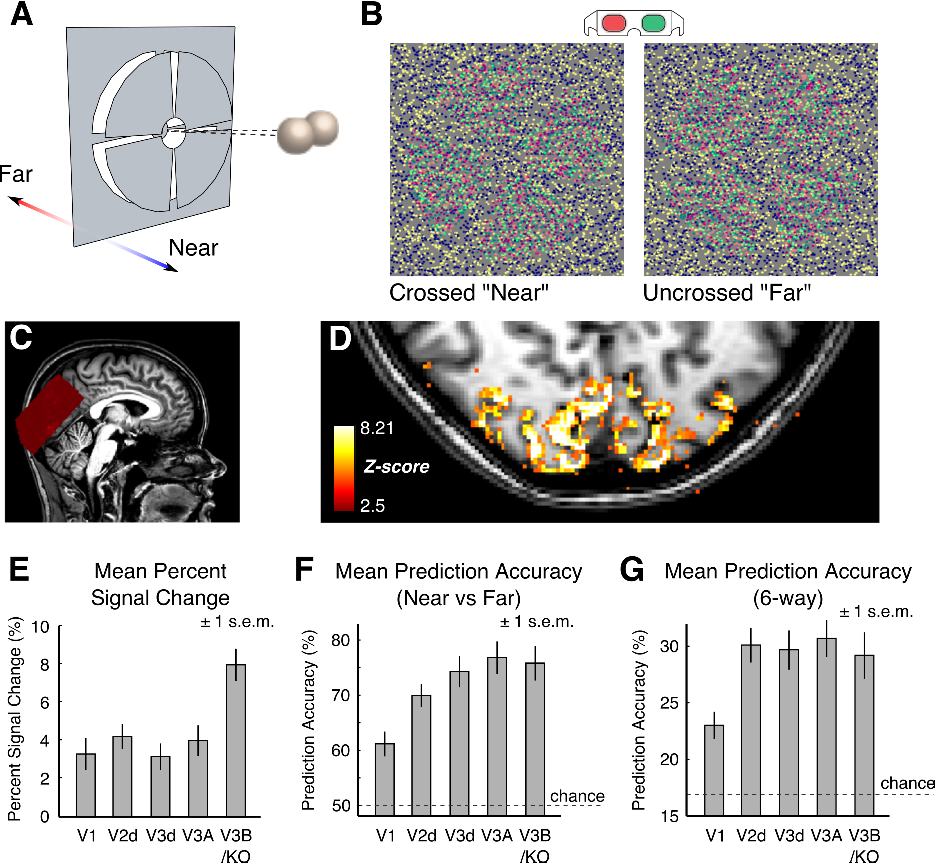
\includegraphics[width=14cm, keepaspectratio]{fig1}
  \caption[Schematic illustration of the stimuli and basic functional activations.]{Schematic illustration of the stimuli and basic functional activations. A, Diagram of the depth arrangement in the stimuli. Four disparity-defined wedges were simultaneously presented at one of six disparity-defined depths during each imaging session ($\pm$ 3, 9 and 15 arcmin in sessions 1 and 2; $\pm$ 12, 24 and 36 arcmin in session 3). B, The depth of the wedges was defined by manipulating disparity in random dot stereograms, which were viewed through red-green anaglyphs attached to prism glasses. C, Blood oxygenation level-dependent signals were acquired from dorsomedial visual cortex. Slice placement is illustrated here on a near mid-sagittal slice in participant 1. D, Signal changes in response to stimulus delivery (stimulus versus rest) for participant 1, showing that activity is localized to the gray-matter. E, Mean percent-signal change for stimulation versus blank periods across all subjects and sessions (N=16). Error bars represent the s.e.m.. F, Mean prediction accuracy for the discrimination of crossed `near' vs. uncrossed `far' disparities across early and dorsal visual areas (two-way classification). Chance level (50\%) is indicated by the dashed gray line. Error bars depict the s.e.m. across subjects and sessions (N=16). G, Mean prediction accuracy for the discrimination of individual disparity conditions presented within each session (six-way classification). Chance performance (16.7\%) is indicated by the dashed gray line. Error bars depict the s.e.m. across subjects and sessions (N=16).}
  \label{fig:ch4fig1}
\end{figure}

\subsection{The spatial clustering of disparity preferences}
Motivated by reports of disparity clustering in macaque extrastriate cortex \cite{Anzai:2011gb,Yeagle_Lafer-Sousa_Conway_2013}, I tested for clustering within the human visual cortex. In particular, I examined the spatial distribution of disparity preferences across the cortical surface by labeling individual voxels according to the disparity value that evoked the highest level of fMRI activity (i.e., maximum beta-weight of the GLM) during each imaging session. To visualize the data, I color-coded the disparity preferences of individual voxels and mapped these preferences onto flattened representations of the cortex. This produced cortical maps with an apparent organization: contiguous spaces across the cortical surface share similar disparity preferences (Fig. \ref{fig:ch4fig2}A,B, top). Importantly, these contiguous areas did not overlap with regions where the mean amplitude of the BOLD signal was low, suggesting that clustering was not a result of macrovascular contributions (Fig. \ref{fig:ch4fig2}A,B, bottom). Moreover, considering disparity preferences at different cortical depths suggested consistent preference, which would be expected for hypercolumn-type organization (Fig. \ref{fig:ch4fig2}C,D; note that the scale of the cortical depth axis here is expanded relative to the cortical location plane to aid visualization).
While these visualizations are useful in illustrating general spatial profiles of responses, the process of mapping and interpolating the data from the (raw) native fMRI data space to a flattened representation of the cortical sheet can introduce over- (or under-) representation of individual datum. In particular, there are frequent one-to-many correspondences between voxels in the functional space and pixels visualized on the flat cortical surface (i.e. oversampling), which can inflate the degree of clustering observed on these flat maps. Therefore, I sought to evaluate preference clustering by examining the disparity response of neighboring voxels in the (native) functional space, thereby ensuring no over- or under- representation of the data. 

\begin{figure}
  \centering
  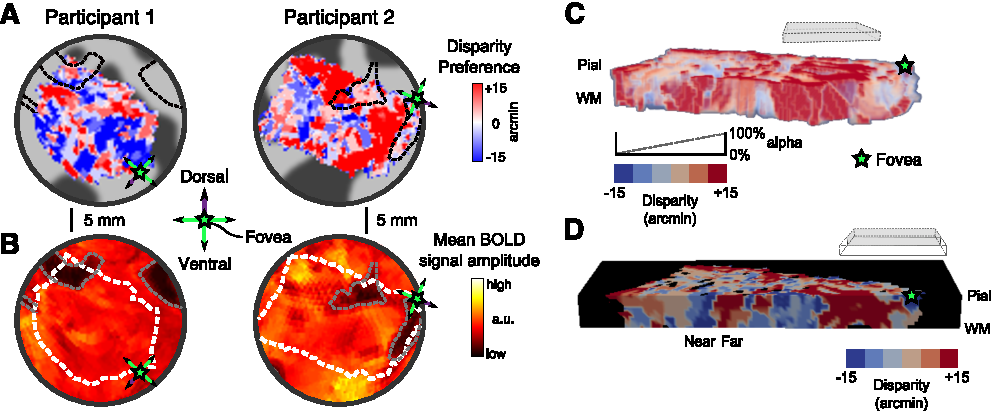
\includegraphics[width=14cm, keepaspectratio]{fig2}
  \caption[Spatial distribution of peak disparity responses in area V3A.]{Spatial distribution of peak disparity responses in area V3A for two participants. A and B, (top) Peak disparity responses in left V3A of participants 1 and 2 (first session). The peak disparity response of each voxel is mapped onto flattened representations of the cortex. Dark and light gray areas represent sulci and gyri, respectively. Peak disparity responses were sampled from three intermediate layers of the cortical sheet (at relative depths of 0.4, 0.5 and 0.6) and averaged across depths. (bottom) Mean BOLD signal amplitude in the same regions of interest. Dark areas indicate low signal amplitude, and are likely to represent large veins. The white dashed line represents the outline of left V3A shown above. Gray dashed lines delineate areas with low signal amplitude in both maps. Coarse clusters of peak disparity responses do not overlap with the potential location of large veins. C, The same ROI in Participant 2, but now represented across 11 relative points through the entire range of the cortical sheet (0 to 1 relative depth, sampled at increments of 0.1). The flattened representations for each cortical depth were stacked together and an opacity gradient was applied to aid visualization of peak disparity response across the cortical depth. Note that to assist visualization the cortical depth, dimension is not drawn to scale. D, Sliced view of peak disparity responses in the same ROI (Participant 2, left V3A). Data are cut through the cortical depth along a line extending from the foveal representation of V3A up to the periphery near the border with V3d.}
  \label{fig:ch4fig2}
\end{figure}

To quantify disparity preference clustering, I assessed the similarity between the preference of a central target voxel and that of its neighbors. I did this by calculating the distribution of disparity preferences in the population of voxels that shared at least one vertex with the target voxel. Thereby, I calculated a probability map for the disparity preference of the neighborhood referenced to the disparity preference of the target voxel (Fig. \ref{fig:ch4fig3}A, for a schematic illustration). My logical expectation was that if there is clustering in the disparity preferences, target voxels will be surrounded by neighbors with the same- (Fig. \ref{fig:ch4fig3}A, top) or similar- (Fig. \ref{fig:ch4fig3}A, middle) preferences, in contrast to randomly organized preferences (Fig. \ref{fig:ch4fig3}A, bottom). However, the extent to which this structure will be visible depends on the spatial scale of the underlying neural maps in relation to the fMRI sampling resolution. Before examining the empirical data, I therefore consider the extent to which clustering can be recovered based on a simulated data set.
To test for clustering at the voxel level, I performed simulations using a model of cortical columns for orientation \cite{ROJER:1990bq}, as there is no standard model for disparity organization. I supposed neural maps of different spatial scales (columns from 1 to 4 mm in width) and then sampled these maps using a simulated 1 mm isotropic `voxel' grid (Fig. \ref{fig:ch4fig3}B). Thereafter, I computed the voxel similarity of each sampled voxel relative to its neighbors, and then averaged together the neighborhood preferences of all voxels that had the same central voxel preference. This resulted in a similarity matrix that shows the statistical relationship between the preference of central voxels relative to their surround (Fig. \ref{fig:ch4fig3}B, bottom), where strong diagonal structure indicates a close relationship between central voxels and their local neighbors. (Note that the higher probabilities in the top left, and bottom right corners of these plots arise because orientation is a circular dimension; one would not anticipate these for binocular disparity which is a more linear dimension). These simulations indicate that using 1 mm isotropic voxels, it is realistic to obtain information about the structure of underlying cortical organization if the scale of the neural maps is in the region of 3 mm. This corresponds to estimated scale of disparity maps in human cortex based on scaling up measurements from macaque MT to account for overall brain size \cite{DeAngelis:1999fk,Ban:2012jr}.
Having demonstrated proof of concept, I now return to the empirical fMRI data. In principle, one could calculate clustering in exactly the same way as described for the simulations. However, real fMRI voxel responses are not temporally or spatially independent, because of the point-spread function (PSF) of the BOLD signal, meaning that a more sophisticated method is required. In particular, I estimated the preference of the (i) central target voxel and (ii) its neighbors using independent data sub-samples (leave-two-out cross-validation), such that shared preferences for a given measurement could not simply be due to the dependency of BOLD responses for nearby voxels. While this strategy does not remove the influence of spatial blurring, it eliminates temporal correlations between neighboring voxels since I use different time-courses for estimating the preference of central voxels and their surround. I computed preference similarity for each presented disparity value, creating matrices for each region of interest (Fig. \ref{fig:ch4fig3}C). I found that diagonal structure in the preference similarity matrices became increasingly apparent for measurements at increasing levels of the dorsal cortical hierarchy. To quantify this observation, I used a reliability statistic that compared the mean probability along the positive diagonal of a matrix, with a distribution of mean values calculated from random sampling from all locations within that matrix (bootstrapping: 10,000 resamples of six values). I found evidence for significant clustering in V2d (p=.04), V3d (p=.01), V3A (p=.02) and V3B/KO (p=.003), but not in V1 (p=.11). As a control, I re-computed matrices after shuffling disparity preferences and found no systematic structure (Fig. \ref{fig:ch4fig3}D). This confirmed that evidence for clustering in higher dorsal areas could not somehow derive from differences in size and/or shape between different regions of interest. Together, these data provide evidence that clustering of disparity preferences is particularly marked in higher dorsal visual areas V3A and V3B/KO in contrast to primary visual cortex. It is possible that preference clustering is much less pronounced in early visual areas. However, recall that from my earlier simulations of maps with different spatial scales, it is possible that there is systematic organization in early areas, but the fMRI sampling resolution does not allow this to be detected.

\begin{figure}
  \centering
  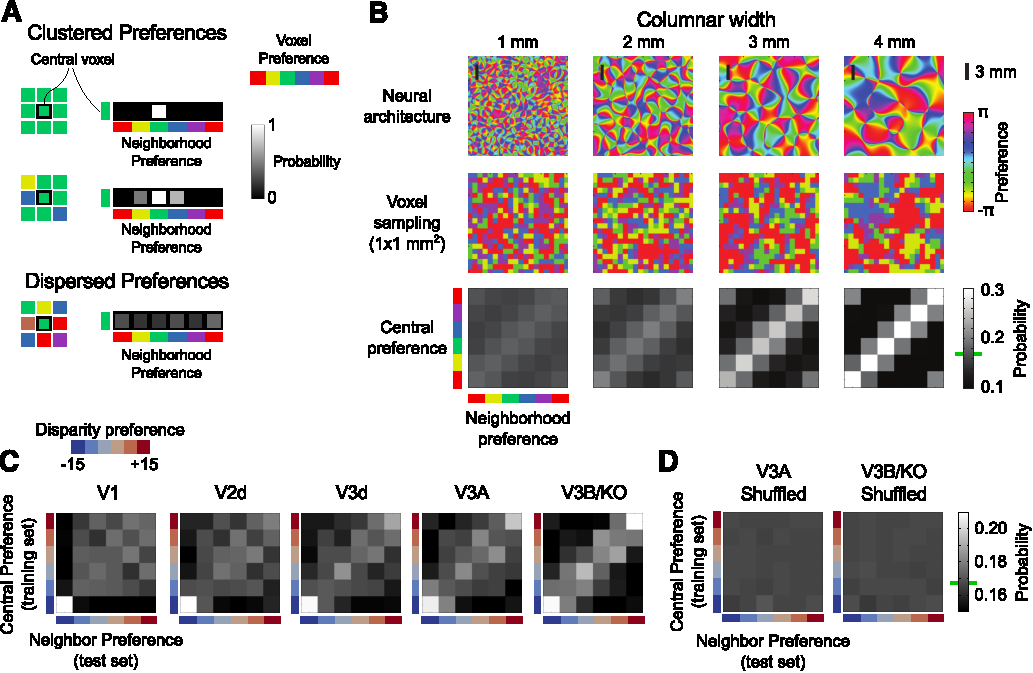
\includegraphics[width=14cm, keepaspectratio]{fig3}
  \caption[Local clustering of peak voxel responses to disparity.]{Local clustering of peak voxel responses to disparity (`preferences') in simulated and empirical data sets. A, Simplified 2D illustration of clustered and disperse preferences for a given voxel. Individual voxels and their neighbors will often share a similar preference if there is spatial clustering (top and middle). If there is no organization, no relationship should be observed between the peak responses of a target voxel and its neighbors (bottom). B, A simulation of columnar architectures for orientation \cite{ROJER:1990bq} with periodicity varying from 1 to 4 mm (top) and the respective preference maps after simulating voxel sampling using six equidistant conditions (middle). Bottom: the correspondence between the preference of target voxels and their neighborhood is shown in form of a probability matrix for each columnar width. In each matrix, the i\textsuperscript{th} row represents the average probability distribution of preferences around voxels preferring the i\textsuperscript{th} disparity, and the probability value is represented in grayscale (green horizontal line on the colorbar indicates chance level, 0.167, given that I have considered six preferences). Maps that are well clustered display a clear diagonal structure, demonstrating that nearby voxels tend to share similar preferences. C, The same matrix representation for empirical disparity maps from visual areas V1, V2d, V3d, V3A and V3B/KO. Green horizontal bar on the colorbar indicates chance level (0.167). A diagonal structure emerges along the dorsal cortical hierarchy. Note the different grey scale range from part B for empirical fMRI measurements. D, Results of a similar analysis after randomly shuffling the disparity preferences in V3A and V3B/KO. In this case, one does not observe any diagonal structure.}
  \label{fig:ch4fig3}
\end{figure}

\subsection{Testing for the reproducibility of disparity preferences}
The preceding analyses support the notion that responses to disparity are clustered in dorsal extra-striate cortex. However, to determine the extent to which this clustering represents genuine cortical structure, I next sought to test whether the spatial distribution of disparity preferences is a persistent property of neuronal responses. Specifically, I tested whether preference maps could be reproduced between different imaging sessions. 
Comparing functional data across different imaging sessions, especially at very high resolution, is extremely challenging, and previous UHF studies have therefore focused on repeatability within sessions \cite{Cheng:2001fk,Yacoub:2008hr}. In particular, differences in voxel slab positioning in relation to the cortical sheet affect sampling \cite{Cheng:2001fk}. Moreover, with a functional resolution of 1 mm (near isotropic), one expects to acquire approximately two points from a given location on the cortical sheet meaning that additional discrepancies could arise from sampling at different cortical depths. As a result, one would not necessarily expect one-to-one voxel correspondence between functional data acquired in different imaging sessions.
Nevertheless, I was able to capture similarities between individual disparity preference maps across sessions for four of the six participants that took part in repeated sessions (Fig. \ref{fig:ch4fig4}A-D). In these maps, disparity preferences appear to be coarsely organized into bands, which can be clearly identified in maps obtained in different imaging sessions (see the outlines in Fig. \ref{fig:ch4fig4}). For one participant (Participant 5, Fig. \ref{fig:ch4fig4}E), I found similar structures across sessions, but with reversed disparity sign (note the correspondence between blue and red regions across sessions, particularly in the right hemisphere). This map inversion is consistent with a change from a rear- to front- projection setting, causing a left-right horizontal flip and thereby reversing the disparity sign presented during the experiment. I suspect that this was the result of restarting the projector immediately prior to this participant's scan due to technical problems. For the final participant, I did not find apparent correspondence between sessions, although I note that slice positioning was not optimal in the second session and a portion of V3A was omitted (Fig. \ref{fig:ch4fig4}F).

\begin{figure}
  \centering
  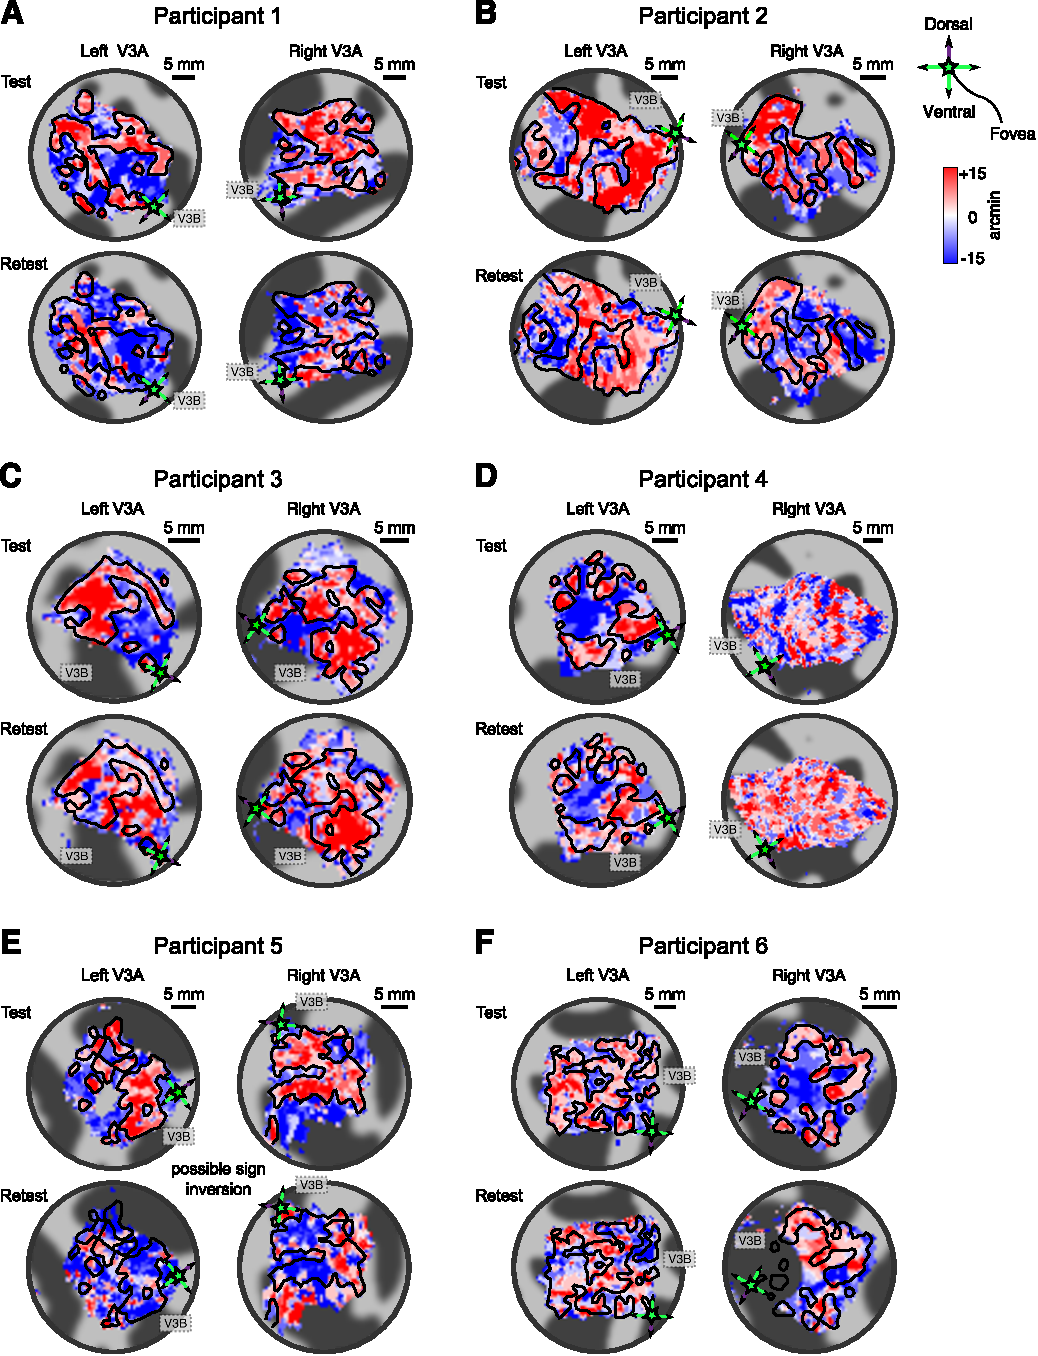
\includegraphics[width=11cm, keepaspectratio]{fig4}
  \caption[Maps of peak disparity responses from area V3A.]{Maps of peak disparity responses from area V3A obtained in different imaging sessions. Flattened representations were obtained by averaging disparity preferences across three intermediate layers in the cortex (0.4, 0.5 and 0.6), so as to avoid distortions caused by macrovasculature near the pial surface. Green pentagrams represent the location of the foveal representation used to identify the border between area V3A and V3B/KO (using retinotopic mapping). The dorsal direction is indicated by the purple arrow aligned with the vertex of the pentagram. Additional labels indicate the position of area V3B/KO to aid orientation. A-D, Persistent distribution of disparity responses can be observed in four participants (Participant 1, left V3A; Participant 2, left and right V3A; Participant 3 right V3A; Participant 4 left V3A). Overlaid contours represent the edges of the uncrossed disparity/`far' (red) region from session 1. These were calculated by binarizing the maps, and then applying an edge detection algorithm. The outlines were omitted in panel D (right V3A) since the fine scale changes in this map mean that superimposed contours masked the data and therefore hindered visualization. E, The distribution of peak disparity responses in participant 5 reveals similar structures between sessions, but the color map appears to be inverted. F, No correspondence between disparity maps is evident for participant 6. Slice positioning in the second session was not optimal, with the result that not all of right hemisphere V3A was fully sampled (bottom right).}
  \label{fig:ch4fig4}
\end{figure}

To quantify the similarity between maps, I used voxel-wise correlation in the native functional space. I first selected voxels that had a stable within-session preference and then brought the functional data from each session into common alignment (see Methods and Materials). I then computed the Pearson correlation between corresponding voxels (nearest neighbors) across sessions using bootstrapped resampling (10,000 samples). Confirming my observations from the flattened cortical representations (Fig. \ref{fig:ch4fig4}), I observed reliable correlations between disparity maps for four participants (Fig. \ref{fig:ch4fig5}A, Participants 1 to 4). In addition, I found reliable negative correlations for one participant (Fig. \ref{fig:ch4fig5}A, Participant 5), in line with the apparent inversion of the disparity maps (Fig. \ref{fig:ch4fig4}E). 

\begin{figure}
  \centering
  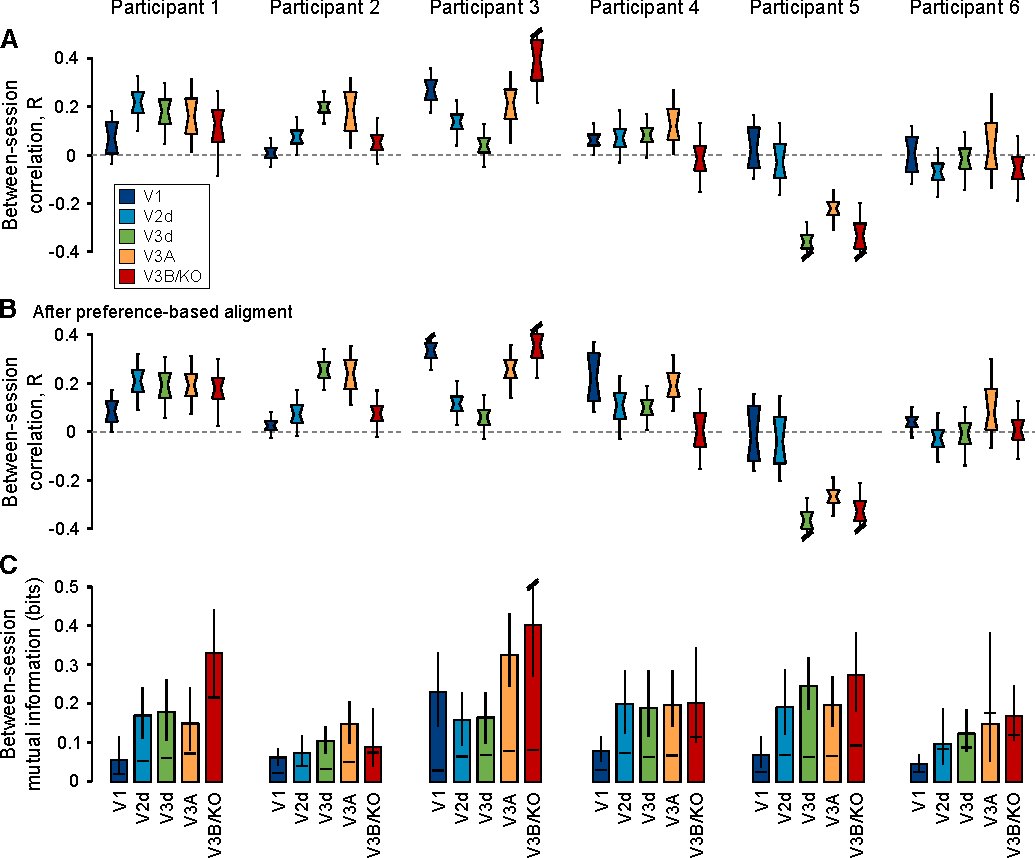
\includegraphics[width=14cm, keepaspectratio]{fig5}
  \caption[Quantifying correspondence between disparity maps.]{Quantifying correspondence between disparity maps acquired in different imaging sessions. A, Correlation between peak disparity responses. Data show the distribution of the Pearson correlation coefficients between voxels' peak responses in session 1 vs. session 2 obtained by bootstrapping (10,000 resamples). The center of the bowties represents the median correlation value. The sides of the bowties and the whiskers extend to the 68\% and 95\% confidence intervals, respectively. Diagonal slashes indicate that the confidence intervals extend beyond the limits of the ordinate axis. B, As A, except that the alignment between the data in the two sessions was improved using an additional alignment procedure. C, Information shared between maps acquired in different sessions. Bars represent the mutual information between maps, with error bars covering the 95\% confidence interval. Horizontal lines represent the 97.5 percentile for a bootstrapped control distribution (10,000 estimates) calculated after randomly shuffling labels of peak disparity response.}
  \label{fig:ch4fig5}
\end{figure}

As discussed above, small spatial misalignments between sessions can lead to an underestimation of between-session repeatability. To ameliorate small misalignments, I considered an additional processing stage in which I incorporated a preference-based between-session alignment step. In particular, I calculated an affine transform between the three-dimensional maps that sought to improve co-registration, while minimizing non-linear deformations (see Methods and Materials). I then recomputed correlations across sessions (Fig. \ref{fig:ch4fig5}B), and found a small improvement in correlation values for participants with previously reliable between-session correspondence. However, the method itself did not introduce significant correlations (e.g. participant 6) when there was little common structure before alignment, and, in general, the effect of this additional alignment step was quite slight. In particular, Figure \ref{fig:ch4fig6} shows the V3A map for participant 4 (that showed the maximum benefit from this alignment step) with and without the additional alignment step. 

\begin{figure}
  \centering
  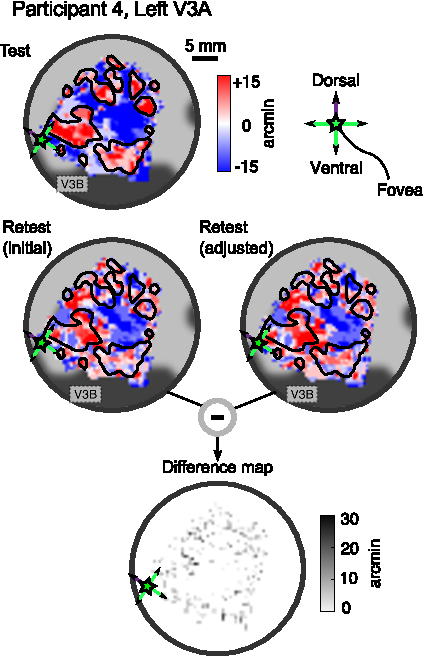
\includegraphics{fig6}
  \caption[Spatial adjustment step.]{Spatial adjustment introduced by the additional alignment step illustrated for participant 3, left V3A, which showed the maximal benefit of this procedure. Top, the map of peak disparity responses obtained in the first imaging session (reproduced from Fig. \ref{fig:ch4fig4}D). Middle, maps obtained in the second imaging session before (left, reproduced from Fig. \ref{fig:ch4fig4}D) and after (right) adjustment using the additional alignment step. Bottom, a difference map illustrating that only minor differences are introduced by the additional alignment step.}
  \label{fig:ch4fig6}
\end{figure}


To provide an additional measure of reproducibility, I computed the mutual information \cite{Shannon1948,shannon1949} between maps obtained in different imaging sessions (using the non-preference-aligned data). I compared the empirical mutual information (Fig. \ref{fig:ch4fig5}C) with bootstrapped estimates based on randomly permuted disparity preferences (Fig. \ref{fig:ch4fig5}C, horizontal lines). I found evidence of persistent information for five participants, confirming the presence of disparity selective structures.

\subsection{Quantifying voxel response profiles at different disparity magnitudes}
In the previous sections, I tested for clustering of disparity preferences by assigning a single disparity preference to each voxel using a winner-takes-all labeling approach. This is an obvious simplification because neurons sensitive to disparity respond to a range of different disparity values. Moreover, disparity tuning curves of individual neurons often vary greatly in morphology --- some neurons may respond to a limited range of disparities, while others respond to many horizontal disparities and are only selective for disparity-sign \cite{Poggio:1988ij,Poggio:1977ys}. In fact, a comprehensive study of disparity tuning properties suggests that neurons can present a wide range of variation in their responses across the disparity domain. In fMRI measurements, voxels aggregate activity of many such neurons, and consequently the response of individual voxels may present an even greater variety of morphologies. I therefore sought to quantify each voxel's response profile to the range of presented disparities. To do so, I first used the tuning templates described by Poggio \cite{Poggio:1988ij,Poggio:1977ys}. These templates offer a descriptive approximation of the response profiles of many disparity selective neurons \cite{DeAngelis:1999fk,Prince:2002uq}, and are simpler (in terms of the number of parameters) than the Gabor models that I will use later. I used these simplified models of disparity selectivity to examine the responses of individual voxels that aggregate the responses of many individual neurons. This voxel-based sampling is quasi-random with respect to the underlying neuronal populations, and, as discussed above, the scale at which underlying neural representations are sampled clearly influences the information available at the voxel level. Nevertheless, on the basis that disparity representations are clustered, it is reasonable to ask whether the local population activity captured by voxels can be related to physiological models of disparity selectivity, and how such models are distributed across the cortical surface. 
I considered three types of selectivity (Fig. \ref{fig:ch4fig7}A): (i) near/far tuned responses (Tuned), (ii) near/far categorical responses (Categorical) and (iii) excitatory and inhibitory tuned responses at zero depth (Zero-tuned). For each voxel, I regressed the selectivity models aligned to the preferred disparity of the voxel (Fig. \ref{fig:ch4fig7}B) against the beta-weight response profile of the voxel. This provided me with a set of three weights and a constant for each individual voxel. I selected voxels whose activity was well captured by the regression approach ($R^2 > 0.8$), resulting in the selection of approximately half the voxels in each ROI (45 $\pm$ 5 \%). Of these selected voxels, I found that 65 $\pm$ 10 \% of the selected voxels were best described as tuned, 15 $\pm$ 6 \% as categorical and 20 $\pm$ 10 \% as zero-tuned (mean $\pm$ standard deviation).

\begin{figure}
  \centering
  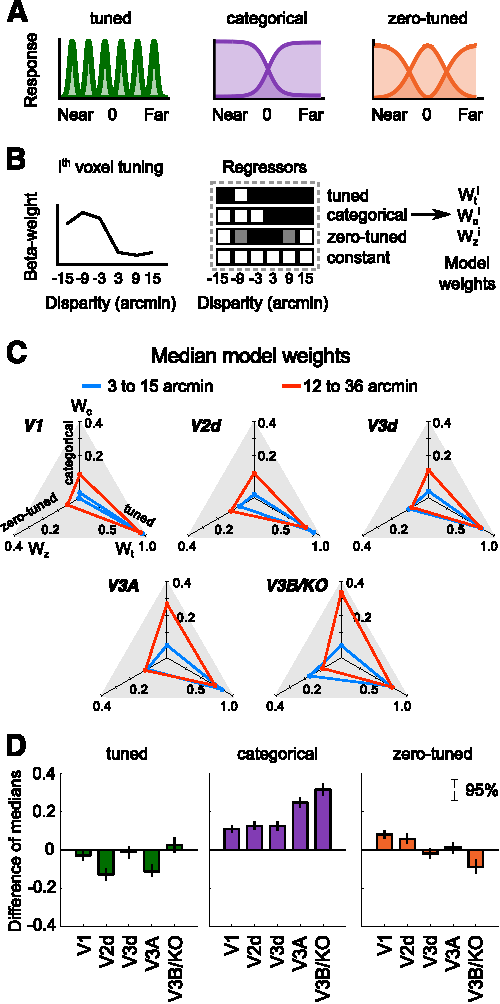
\includegraphics{fig7}
  \caption[Modeling voxel responses using simplified models of disparity selectivity.]{Modeling voxel responses using simplified models of disparity selectivity. A, A representation of the descriptive models of disparity selectivity proposed by Poggio et al. \cite{Poggio:1988ij}. B, Schematic representation of the model-based approach. For each individual voxel, I assembled regressors based on the hypothetical responses for each model type given the peak disparity response of the voxel. After linear regression, I obtain three weights that approximate the contribution of each model for the response profile of individual voxels. C, Model weights at different disparity magnitudes. The median weights (across voxels) for each model are mapped onto a radar plot with three axis (one for each model). Blue lines represent data from the first two imaging sessions (pooled), during which disparity ranged from 3 to 15 arcmin. Red lines represent the distribution of weights observed at disparities ranging from 12 to 36 arcmin (third session). D, Difference in medians between the distributions illustrated in C for all regions of interest. Bars represents the median difference (in medians) obtained by bootstrapping (10,000 resamples). Error bars represent 95\% confidence intervals.}
  \label{fig:ch4fig7}
\end{figure}

Psychophysical investigations and models of stereoacuity suggest that the selectivity of perceptual disparity detectors varies with disparity magnitude --- at increased disparity magnitudes, disparity detectors have broader response profiles \cite{Stevenson:1992kx,Lehky:1990fk}. This led me to hypothesize that such a relationship would be reflected in the representation of `tuned' and `categorical' responses at different disparity magnitudes. Particularly, I predicted that increasing the disparity magnitude of stimuli could lead to an increase in the amount of categorical responses in areas that may be closely related to stereopsis. To test this, I ran an additional experiment with a larger range of disparities. Four participants undertook a third imaging session, during which disparity was varied between 12 and 36 arcmin (crossed and uncrossed). I then used the model-based analysis of the voxel responses to test whether estimated profiles were affected by the increase in disparity magnitude. Specifically, I pooled the data across subjects for each disparity range, and computed the median weight of each model (across voxels). Using this approach, an increased representation of a particular model is demonstrated by an increase in the weight assigned to that model by the regression approach. I visualized the weight for each model in a radar plot with three axes, one for each response model (Fig. \ref{fig:ch4fig7}C), and found an increased representation of categorical responses at greater disparity magnitudes, especially in areas V3A and V3B/KO (Fig. \ref{fig:ch4fig7}C, compare red versus blue lines; Fig. \ref{fig:ch4fig7}D, purple elements). In other words, a greater proportion of the voxels are best explained by the categorical model when the range of presented disparities was larger. This increase in weights for the categorical model was accompanied by small changes in the distribution of tuned and zero-tuned weights (Fig. \ref{fig:ch4fig7}D, green and orange elements). 
Having estimated the type of response profile exhibited by individual voxels, I next sought to determine if there was any structure in the way in which these voxels are distributed across the cortical surface. In particular, I mapped the weights for each selectivity model onto a representation of cortical surface for each individual (Fig. \ref{fig:ch4fig8}-\ref{fig:ch4fig9}). I found three important features in these maps. First, I observed clustering in the weight maps, indicating that nearby voxels share similar disparity response profiles (e.g., voxels described each model are clustered together on the cortex, as shown by co-localized saturated colors). Second, the cortical locations described by categorical vs. tuned models appear to be distinct (Fig. \ref{fig:ch4fig8}-\ref{fig:ch4fig9}, note the complementarity of the green vs. purple maps within-session). Third, the consistency across all sessions was particularly marked for categorical disparity processing model (compare purple maps across sessions one to three, particularly evident in Fig. \ref{fig:ch4fig8}A, but also apparent for the other participants), with enhanced categorical representations in session three as expected from the wider disparity range. By contrast, for the tuned and zero-tuned disparity models, I only observed correspondence across the first two sessions in which exactly the same disparity levels were tested (Fig. \ref{fig:ch4fig8}B and \ref{fig:ch4fig9}A). This highlights the systematic organization of disparity representations, and makes clear that `tuned' responses are very sensitive to the exact disparity presented, while `categorical' responses show tolerance to the disparity value.

\begin{figure}
  \centering
  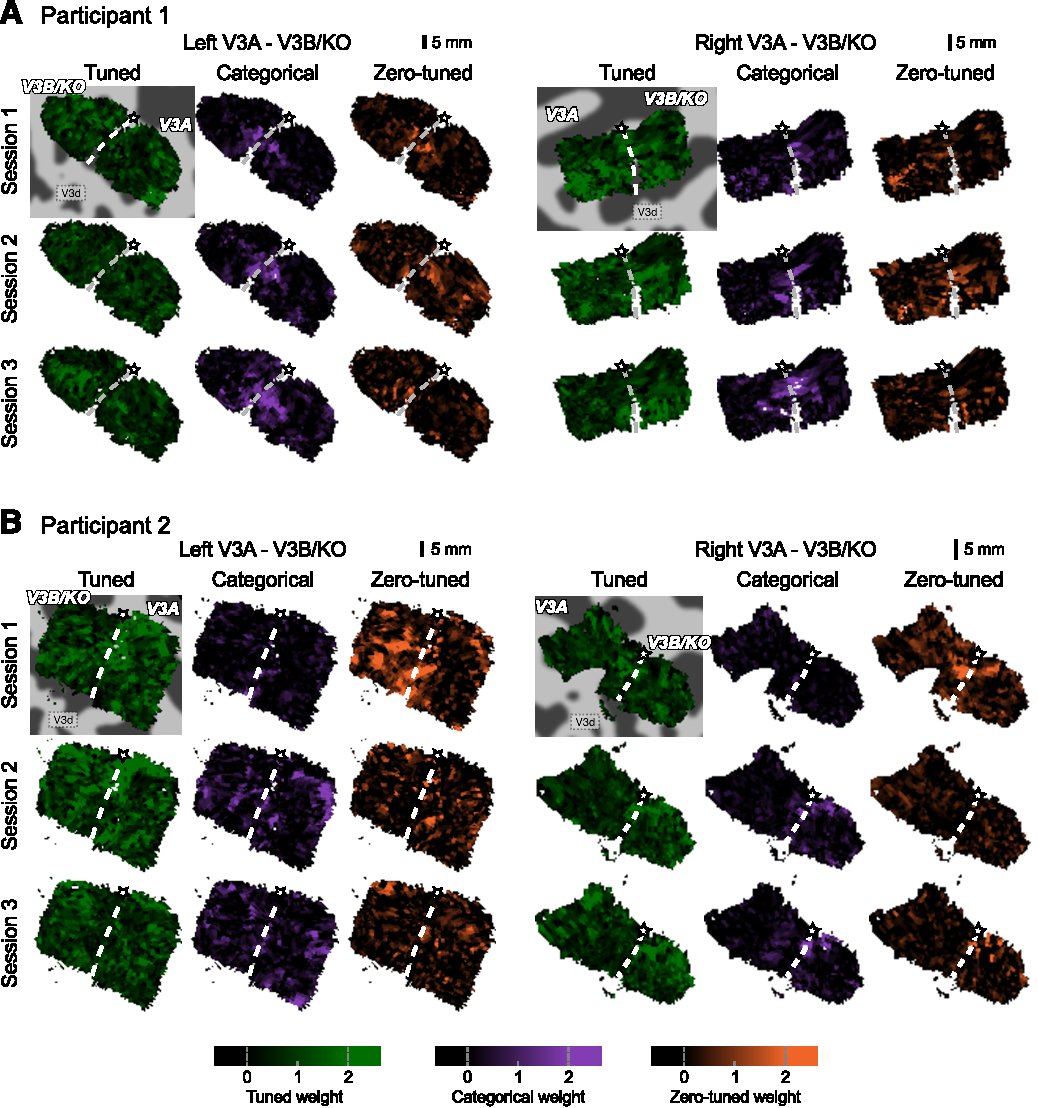
\includegraphics[width=14cm, keepaspectratio]{fig8}
  \caption[Cortical representation of models weights for participants 1 and 2]{Cortical representation of models weights in areas V3A and V3B/KO in the left and right hemispheres of participant 1 (A) and 2 (B). The pentagram on each map represents the position of the fovea, and the white dashed line the division between V3A and V3B/KO established using retintopic mapping. A, Categorical responses (purple) were persistently identified around the foveal representation dividing V3A and V3B/KO (both hemispheres), even when different disparity levels were presented (session 3). B, An apparent correspondence between tuned responses was found across sessions 1 and 2, but not session 3 (left hemisphere).}
  \label{fig:ch4fig8}
\end{figure}

\begin{figure}
  \centering
  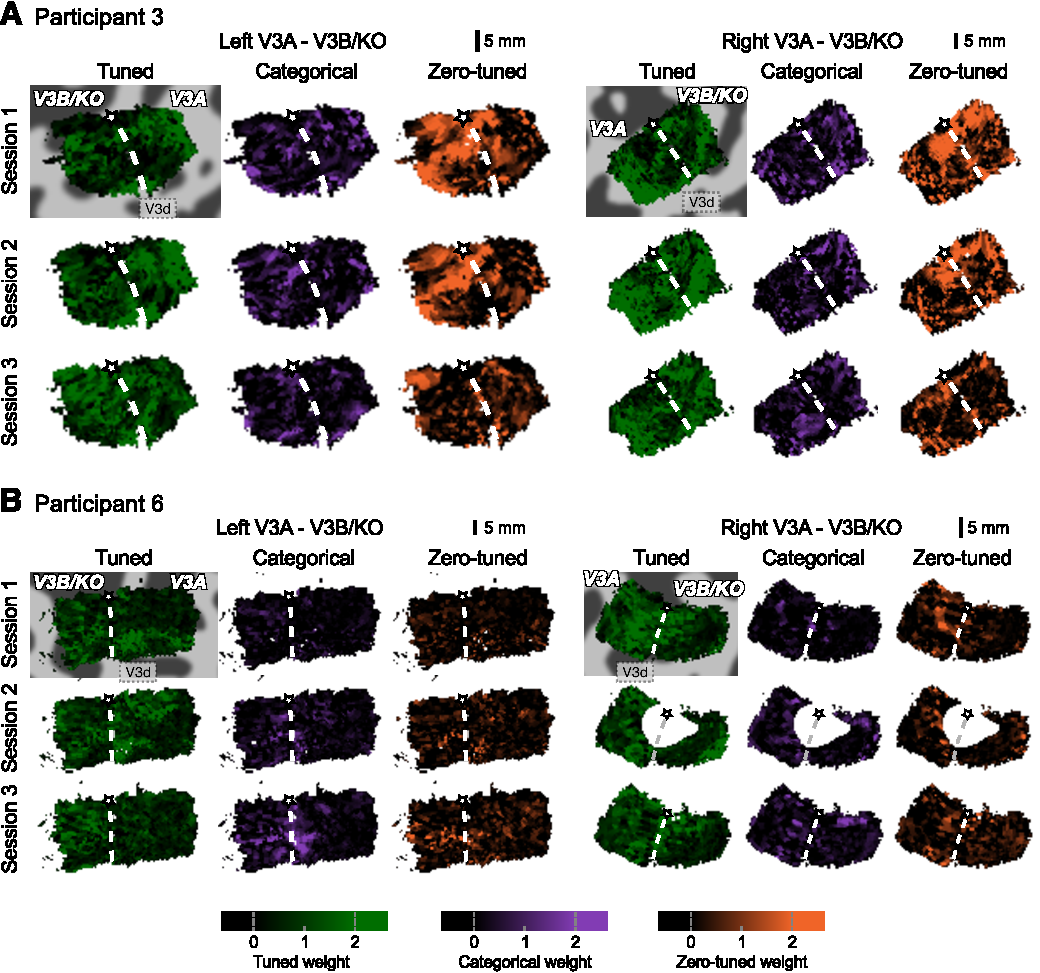
\includegraphics[width=14cm, keepaspectratio]{fig9}
  \caption[Cortical representation of models weights for participants 3 and 6]{Cortical representation of models weights in areas V3A and V3B/KO in the left and right hemispheres of participant 3 (A) and 6 (B). This figure follows the format presented in Figure 8. A, Evident correspondence between `tuned' and `zero-tuned' weights was identified across the first two imaging sessions. That correspondence is not observed for the third session, where disparity magnitude was increased. B, Apparent correspondence was absent for participant 6. Note that the voxel slice placement for session 2 meant that a considerable portion of V3A and V3B/KO in the right hemisphere was not covered.}
  \label{fig:ch4fig9}
\end{figure}

Our data analysis so far has employed relatively simplistic models of disparity selectivity to describe the responses of individual voxels. Biases in the representation of these models indicated an increase in categorical responses when participants viewed stimuli at higher disparity magnitudes. Next, I sought to examine this relationship in greater detail by fitting physiologically-inspired models of disparity selectivity. In particular, I asked whether changes in voxel response width could be observed between groups of voxels preferring different disparity magnitudes. 
For each region of interest, I grouped voxels according to their peak disparity response (3, 9, 12, 15, 24 and 36 arcmin, crossed and uncrossed), and then fit a Gabor tuning profile models to each of these twelve groups. Figure \ref{fig:ch4fig10}A shows representative responses of voxels with maximal responses for $-$3, 12, 15 and 36 arcmin, in three different ROIs. For the higher dorsal areas, I observe that the Gabor fit (black line) to the response profile is broader for large disparities than it is for small disparities. I quantified this using the standard deviation (SD) parameter of the Gabor model, plotting this as a function of the peak response of the voxels (Fig. \ref{fig:ch4fig10}B). In early visual areas (V1, V2, V3d) I found that the width of voxels' response profiles was not related to the overall disparity magnitude. By contrast, in areas V3A and V3B/KO I observed significant relationships between the peak disparity response and the width of the Gabor fit.
One potential concern with this analysis is that such a relationship may be a consequence of the differential spacing between the presented disparities in different imaging sessions, i.e. the envelop width is broader because of the wider stimulus spacing. Ideally, I would have used a fine spacing of disparities across a broad range of disparity magnitudes, which would rule out such a concern. However, the practicalities of obtaining a sufficient number of fMRI measurements within a time-constrained imaging session meant one could not do this. Nevertheless, I judge it unlikely that stimulus spacing {\it per se} accounts for the relationship I observe. First, I did not observe significant correlations in V1 to V3d, suggesting that the increase in disparity spacing alone does not result in a relationship between the peak and SD parameters. Second, I can contrast profiles for overlapping points in this space (Fig. \ref{fig:ch4fig10}a): the width of the fit to the $-$15 tuned units (from sessions 1 and 2 with 6 arcmin stimulus spacing) is wider than for $-$12 (from session 3 with 12 arcmin stimulus spacing). 

\begin{figure}
  \centering
  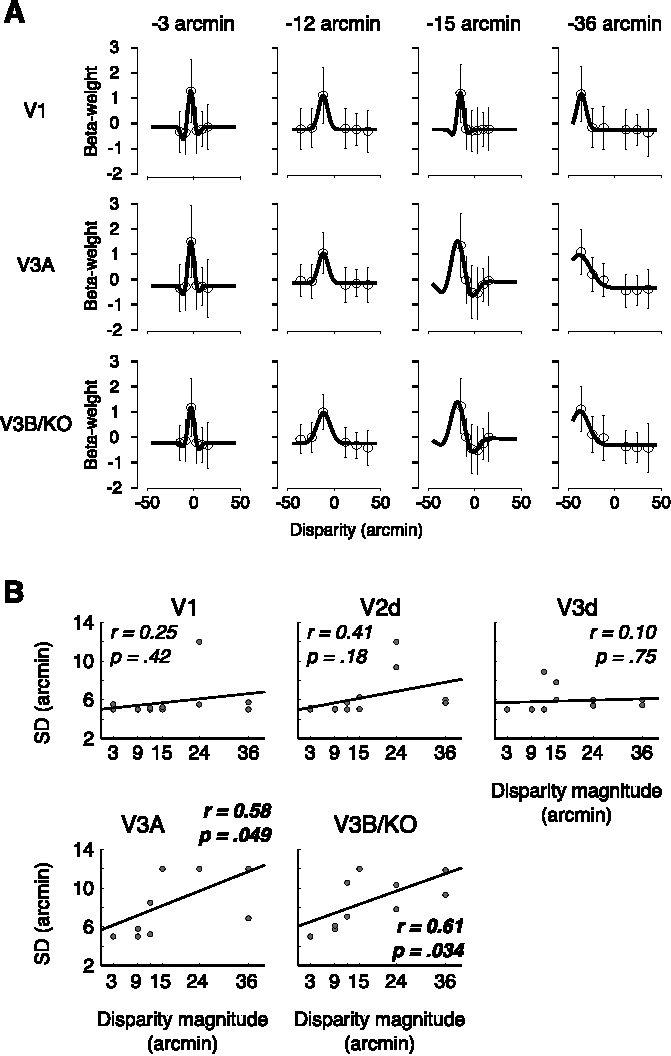
\includegraphics{fig10}
  \caption[Voxel response profiles at different disparity magnitudes.]{Voxel response profiles at different disparity magnitudes. I modeled voxel responses using Gabor filters, and examined the relationship between the Gabor parameters and preferred disparity magnitude. A, Pooled voxel responses in areas V1, V3A and V3B/KO modeled by Gabor filters for four preferred disparities ($-$3, $-$12, $-$15 and $-$36 arcmin). Gabor models were fit to sets of voxels sharing the same preferred disparity, resulting in twelve groups per ROI. Error bars represent the standard deviation across voxels. B, Relationship between response profile width (standard deviation of the Gaussian envelope) and peak disparity response for early and dorsal visual areas. Each datum represents a group of individual voxels that share the same disparity preference (one of the twelve preferred disparities examined in the experiments: $\pm$ 3, 9, 12, 15, 24 and 36 arcmin). A significant positive trend between tuning width and disparity magnitude was found in V3A and V3B/KO, but not in earlier visual areas.}
  \label{fig:ch4fig10}
\end{figure}

Changes in selectivity as a function of disparity magnitude are thought to be characteristic of neural populations that underlie human stereoscopic judgments \cite{Lehky:1990fk, Stevenson:1992kx} (Fig. \ref{fig:ch4fig11}A). Based on fMRI measurements, I sought to test how well estimates of human neural population responses to disparity could account for depth discrimination thresholds. To this end, I built a population of disparity-tuned units based on the estimated (linear) relationship between Gabor parameters and disparity magnitude (Fig. \ref{fig:ch4fig11}B). Using these values suggested that V1 responses were unlikely to account for disparity discrimination judgments (Fig. \ref{fig:ch4fig11}B), however, estimated populations in V3A and V3B/KO produce discrimination threshold curves that are qualitatively similar to previously reported behavioral results \cite{Badcock:1985ly} (Fig. \ref{fig:ch4fig11}C,D) and stereo acuity modeling \cite{Lehky:1990fk} (Fig. \ref{fig:ch4fig11}A). While the overall shape of the curves are similar, a closer fit would likely require testing a wider range of disparities to account for the flanks of the curves, and denser sampling near the fixation point to capture the fine trough near zero disparity. Stevenson et al. \cite{Stevenson:1992kx} use psychophysical measurements to describe the relationship between tuning width of the perceptual mechanisms (parameterized as the full width at half maximum, FWHM) and disparity magnitude. Using data extracted from their paper, and the linear relationship they estimated, I plotted fMRI estimates of voxel response width (FWHM) together with their data and estimated linear relationship (Fig. \ref{fig:ch4fig11}E). This suggests a striking similarity between perceptual- and fMRI- estimates of variations in the tuning of units that respond to binocular disparity. Together, these results suggest an intriguing analogy between activity in V3A and V3B/KO and depth judgments (consistent with previous neuroimaging studies \cite{Preston:2008dg,Ban:2012jr,Murphy:2013ys,Dovencioglu:2013zr}). 

\begin{figure}
  \centering
  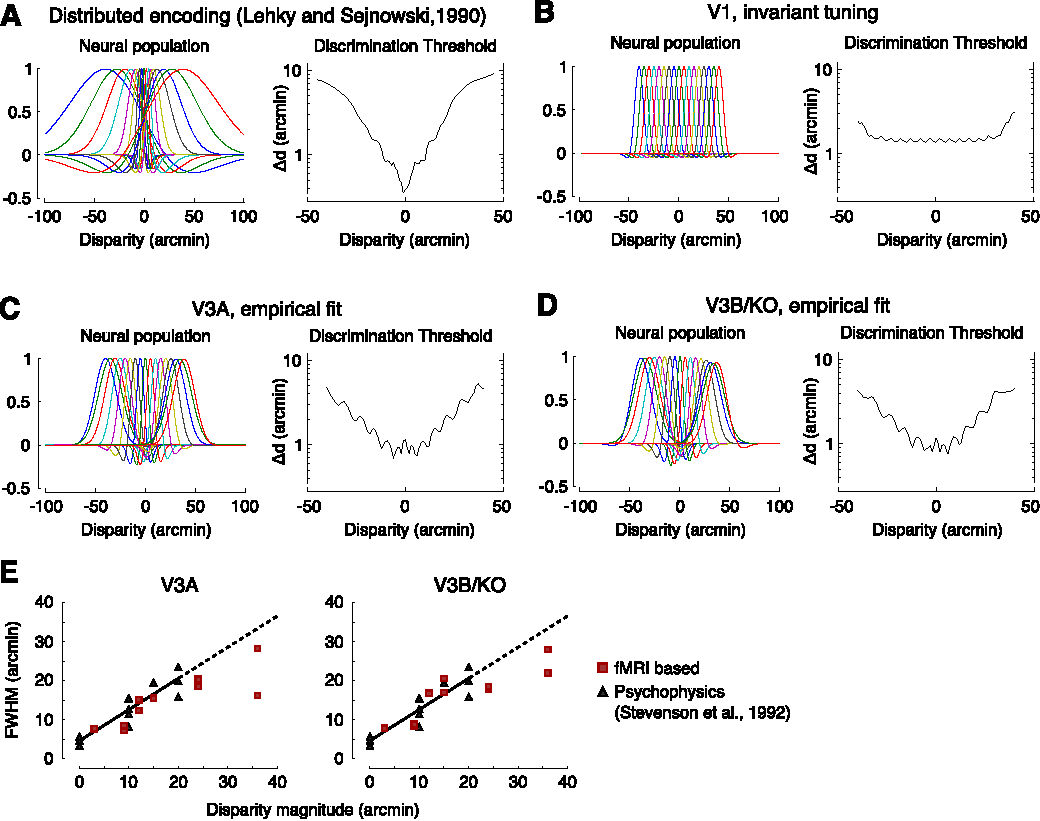
\includegraphics[width=14cm, keepaspectratio]{fig11}
  \caption[Population encoding mechanisms and stereo acuity at different disparities.]{Population encoding mechanisms and stereo acuity at different disparities. A, Distributed encoding model proposed by Lehky and Sejnowski \cite{Lehky:1990fk}. A population of seventeen non-uniform, largely overlapping units (left) produces a disparity discrimination curve (right) similar to stereoacuity judgments made by human observers \cite{Badcock:1985ly}. B, Interval encoding model derived from voxel response profiles in V1. A population of seventeen units with uniform, narrow tuning produces a disparity discrimination curve uncharacteristic of the human visual system. C, D, A neural encoding model derived from the voxel response profiles in areas V3A and V3B/KO (left), and the simulated discriminative performance of these models (right). The performance of these models is more similar to the idealized patterns of psychophysical performance (part A) than a model derived from V1 activity (part B). E, Plot of disparity magnitude against detector tuning width based on psychophysical data published by Stevenson et al.\cite{Stevenson:1992kx}, and fMRI estimates in V3A and V3B/KO. The trend line reproduces that fit by Stevenson and colleagues, with black data points representing their published data (their Figure 7) as obtained by a `data thief' procedure implemented in Matlab. Red data points represent fits from fMRI measurements. The dashed portion of the fit extends the line of best fit beyond the range of disparities tested by Stevenson et al.\cite{Stevenson:1992kx}}
  \label{fig:ch4fig11}
\end{figure}

\section{Discussion}
Here I use 7 T fMRI to test whether human dorsomedial visual cortex contains systematic organized representations of binocular disparity. Using a series of computational modeling approaches, I report three main advances in understanding disparity organization in the human brain. First, I show that disparity preferences are systematically organized (Figs. \ref{fig:ch4fig3}C, \ref{fig:ch4fig4}, \ref{fig:ch4fig8}, \ref{fig:ch4fig9}), and importantly that these preferences are persistent between imaging sessions (Figs. \ref{fig:ch4fig4}, \ref{fig:ch4fig5}, \ref{fig:ch4fig8}, \ref{fig:ch4fig9}). Second, I observed differences between the local distribution of disparity responses in early and dorsomedial visual areas (Figs. \ref{fig:ch4fig3}C, \ref{fig:ch4fig7}, \ref{fig:ch4fig10}), suggesting different properties of cortical organization. Third, by modeling the responses of individual voxels, I show a relationship between tuning width and disparity magnitude (Fig. \ref{fig:ch4fig10}B), indicating more broadly tuned responses to larger disparities, in line with psychophysical and modeling work that posits such a relationship as a characteristic property of neural populations involved in stereopsis (Fig. \ref{fig:ch4fig11}). Together, these findings indicate that human V3A and V3B/KO contain selective cortical structures that are likely to be important in stereoscopic depth processing.
The cortical organization of disparity preferences
Understanding of the cortical structures that support disparity processing is largely informed by recordings in the macaque brain. For instance, by systematically assessing disparity preferences at locations across the cortical surface of area MT/V5, DeAngelis and Newsome \cite{DeAngelis:1999fk} demonstrated smooth changes in preferred disparity across the cortex that indicate systematic organization. More recent electrophysiological evidence indicates that other dorsal visual areas, including V3A, contain clustered representations of disparity \cite{Anzai:2011gb,Yeagle_Lafer-Sousa_Conway_2013}. Based on previous human imaging work \cite{Backus:2001ly,Preston:2008dg}, dorsomedial visual cortex was likely to show strong responses to disparity-defined stimuli in human participants. I find evidence that similar disparities are clustered together, particularly in areas V3A and V3B/KO (Fig. \ref{fig:ch4fig3}C), and that correspondence between maps can be observed even when the presented disparities differ (Fig. \ref{fig:ch4fig8}-\ref{fig:ch4fig9}, categorical responses). While I have concentrated on area V3A, it is interesting that these findings suggest cortical organization for disparity that is similar in its basic properties to macaque MT. Although these two areas appear to have distinct functional properties for binocular disparity \cite{Cottereau:2011uq}, they receive a large portion of inputs from common areas \cite{Felleman:1991kg}. In particular, MT and V3A receive inputs from V2 and V3, where disparity organization has previously been reported \cite{Roe:1995ys,Chen:2008vn,Adams:2001wt,Anzai:2011gb}. Therefore, it is possible that cortical organization for binocular disparity in dorsomedial areas and MT is derived from their downstream inputs in the cortical hierarchy.
While these imaging data suggests clustered responses, it is clearly not possible to infer that the underling organization is columnar. For instance, it is possible that the persistent structures I observe across sessions represent a coarser spatial bias in disparity responses, rather than a periodic columnar structure. Nevertheless, it is encouraging that I observed a difference between dorsal visual areas and responses in primary visual cortex. This appears consistent with macaque electrophysiology in suggesting V1 has only a weak tendency for clustering \cite{LeVay:1988ve,Prince:2002cr}. 

\subsection{Benefits and limitations of UHF imaging for mesoscopic mapping}
Our understanding of cortical organization to date is predominantly informed by animal models, typically using neurophysiological and optical imaging methods that provide a high level of detail, at cost of invasiveness. Recent advances in ultra-high field fMRI make it possible to investigate mesoscopic properties of the human cortex non-invasively \cite{Cheng:2001fk,Yacoub:2008hr,Zimmermann:2011kl}. However, issues in the interpretation of neuroimaging data are usually introduced by (i) potential biases from large vascular structures, which are poorly related to local cortical activity and (ii) insufficient spatial resolution. Here, UHF fMRI revealed that disparity preference representations are well clustered in human dorsal visual cortex. While one may be able to map disparity preferences at lower spatial resolution, the increased BOLD CNR of UHF is likely a requirement to do so. By imaging at UHF, the contributions from large vessels, which could mask the actual distribution of disparity preference, are reduced \cite{Gati:1997uq,Ogawa:1998fk,Ugurbil:2003uq}. This gain in spatial specificity is the fundamental benefit for mapping genuine properties of neural subpopulations.
Although UHF imaging improves spatial specificity, additional care is necessary to avoid the influence of large vessels, especially when mapping functional data onto cortical flattened maps: mapping large veins onto flat maps can result in the emergence of spurious structures unrelated to local activity. I therefore chose to sample functional activity predominantly from the central layers of the cortex in order to avoid large surface vessels \cite{Zimmermann:2011kl,SanchezPanchuelo:2012jq}, and improve spatial localization \cite{Polimeni:2010fl}. This is particularly important given that I used a gradient-echo sequence, which is more susceptible to surface macrovascular contributions compared to spin-echo based sequences \cite{De-Martino:2013wl}. Additionally, I verified that regions where the mean BOLD amplitude was higher (which could derive from larger vessels) were not co-localized with coarser structures found in preference maps (Fig. \ref{fig:ch4fig2}A,B).
Finally, it is necessary to consider the possibility that clustering is enhanced by the point-spread-function (PSF) of the 3D GE-EPI sequence. The PSF of the BOLD signal can reach 2 mm in extent (Gaussian FWHM) \cite{Shmuel:2007hs}, meaning that voxel responses may be significantly influenced by the activity of their neighbors. However, it is unlikely that the PSF is a major barrier to the interpretation of these data. First, even a sequence with a broad PSF can be used to map cortical properties, provided that the contrast-to-noise (CNR) is sufficient \cite{Yacoub:2008hr}. Second, limiting analyses to voxels from central layers of the cortex (i.e., away from large draining vessels on the cortical surface) is likely to have reduced the spatial spread of the BOLD response \cite{Polimeni:2010fl}. Finally, these data point to differences in disparity clustering between visual areas (Fig. \ref{fig:ch4fig3}c). This suggests that the measurement approach has sufficient dynamic range that one can capture changes related to the underlying structure of the cortical organization.

\subsection{Disparity selectivity and stereopsis}
Models of human stereo acuity have posited a relationship between the tuning width of disparity sensitive units as a function of the magnitude of disparity: i.e., neurons selective for fine disparities have smaller receptive fields, while units preferring coarser disparities have larger receptive fields (Fig. \ref{fig:ch4fig11}A; \cite{Lehky:1990fk}). Psychophysical measurements support this conclusion \cite{Stevenson:1992kx}. In this study, I found that the population-estimated responses in human V3A and V3B/KO follow this relationship, and a model based on fMRI estimated tuning widths as a function of presented disparity is able to discriminate disparities in a manner similar to the human visual system. This is captured by the slope of the disparity discrimination curves between small and large disparity magnitudes for V3A and V3B/KO (Fig. \ref{fig:ch4fig11}C,D), resulting in greater stereo acuity for fine rather than coarse disparities. Conversely, a population with invariant tuning properties produces nearly constant disparity discrimination thresholds, implying constant stereo acuity for a wide range of disparity magnitudes (Fig. \ref{fig:ch4fig11}B)
In order to examine disparity responses, I used well-defined tuning templates to group voxels according to their response type (e.g. tuned vs categorical). These templates can be seen as simplifications of the tuning classes suggested by Poggio and colleagues more than two decades ago \cite{Poggio:1988ij}. Since then, it has been suggested that disparity selectivity is better described by Gabor models whose (continuous) parameter space explains previously posited discrete types of disparity tuning \cite{Prince:2002uq}. When I used Gabor models to describe the voxel responses for each disparity level, I found that changes in the envelope width along the disparity domain can be well approximated by a linear function (Fig. \ref{fig:ch4fig11}E; consistent with psychophysical investigations \cite{Stevenson:1992kx}), suggesting that tuning width varies gradually with disparity magnitude (at least within the range tested in this study). 

\section{Conclusion}
Using 7 T fMRI, I show that human dorsal visual areas contain systematically organized structures for disparity processing. The responses of these structures vary with disparity magnitude, which aligns well with previous quantifications of stereoscopic perceptual judgments. Together, these results suggest that areas V3A and V3B/KO contain selective, organized structures that support stereoscopic processing in the human brain.



%%% Local Variables: 
%%% mode: latex
%%% TeX-master: "../thesis"
%%% End: 
